\documentclass[11pt]{scrartcl}
\usepackage[utf8]{inputenc}
\usepackage[english]{babel}
\usepackage{hyperref}
\usepackage{graphicx}
\usepackage{listings}
\usepackage{xcolor}

% COLORS
% Use these definitions to change the color in the listings
\definecolor{green}{rgb}{0,0.6,0}

% CODE LISTINGS
\lstset{
    language=SQL,
    basicstyle=\footnotesize,
    commentstyle=\color{green},
    keywordstyle=\color{blue},
    numbers=left,
    numberstyle=\tiny\color{gray}
}

% biibliography 
% for citation styles see here: 
% https://www.overleaf.com/learn/latex/Natbib%20citation%20styles
%
% You can export references as bibtex (i.e. on google scholar) and copy them to the bibliography.bib
% The most important citation commands are: 
%   \citep{ref} for parenthesis
%   \citet{ref} for a text citation
\usepackage{natbib}
\bibliographystyle{abbrvnat}
\setcitestyle{authoryear,open={(},close={)}}

\newcommand\wordcount[1]{
    \immediate\write18{texcount -sum=[1,0,0] -sub=section #1.tex  | grep "Section" | sed -e 's/+.*//' | sed -n \thesection p > ./\jobname-words.sum}%
    \medskip\par\input{./\jobname-words.sum} words
}

% CHANGE TO YOU NEEDS HERE
\title{SQL Report: Your title goes here}
\author{Your Name}
\date{January 2021}

\begin{document}

\maketitle

\begin{abstract}
    An abstract is absolutely not necessary and you can simply drop or comment this part.
    Alternatively, you can use it to place your contact details:\medskip\par 
    \begin{tabular}{lc}
       student-id  & 1234567 \\
        e-mail & mail@example.com
    \end{tabular}
\end{abstract}

\section{Temperature indices}

\subsection{SQL code}
An overview of temperature indices was implemented using a \texttt{VIEW} as defined in lising \ref{lst:view_1}

\lstinputlisting[label={lst:view_1},caption={create statement for view},]{./sql/temperature_indices.sql}

\subsection{discuss}

% REPLACE WITH YOUR TEXT HERE
In the next paragraph discuss the differences between the Postgres and R solution for calculating temperature indices. 
Name a few advantages \textbf{and} disadvantages for both solutions. 

% this does not yet work...
%\wordcount{main}


\section{Verify results}

% REPLACE WITH YOUR TEXT HERE
Compare your SQL calculated indices to the R calculated indices. Do they differ and if they do, why?

%\wordcount{main}

\section{Spatial variability}

% REPLACE WITH YOUR TEXT HERE
Describe the variability of your sensor compared to the others this year. 
You might also want to place some citations. Check out the comments in the source 
\texttt{main.tex} for the commands. 
If you want to cite your HOBO report here, add an bibliography entry to the \texttt{bibliography.bib} like:

\begin{verbatim}
@article{hobo,
    author={Bar Foo},
    year=2021,
    journal={Data collection, -management, -visualization lecture},
    title={HOBO Report}
}
\end{verbatim}

You can cite it with the \texttt{\textbackslash citep\{hobo\}} command \citep{hobo}.

%\wordcount{main}


\section{Indices across time and space}

\begin{figure}[ht]
    \centering
    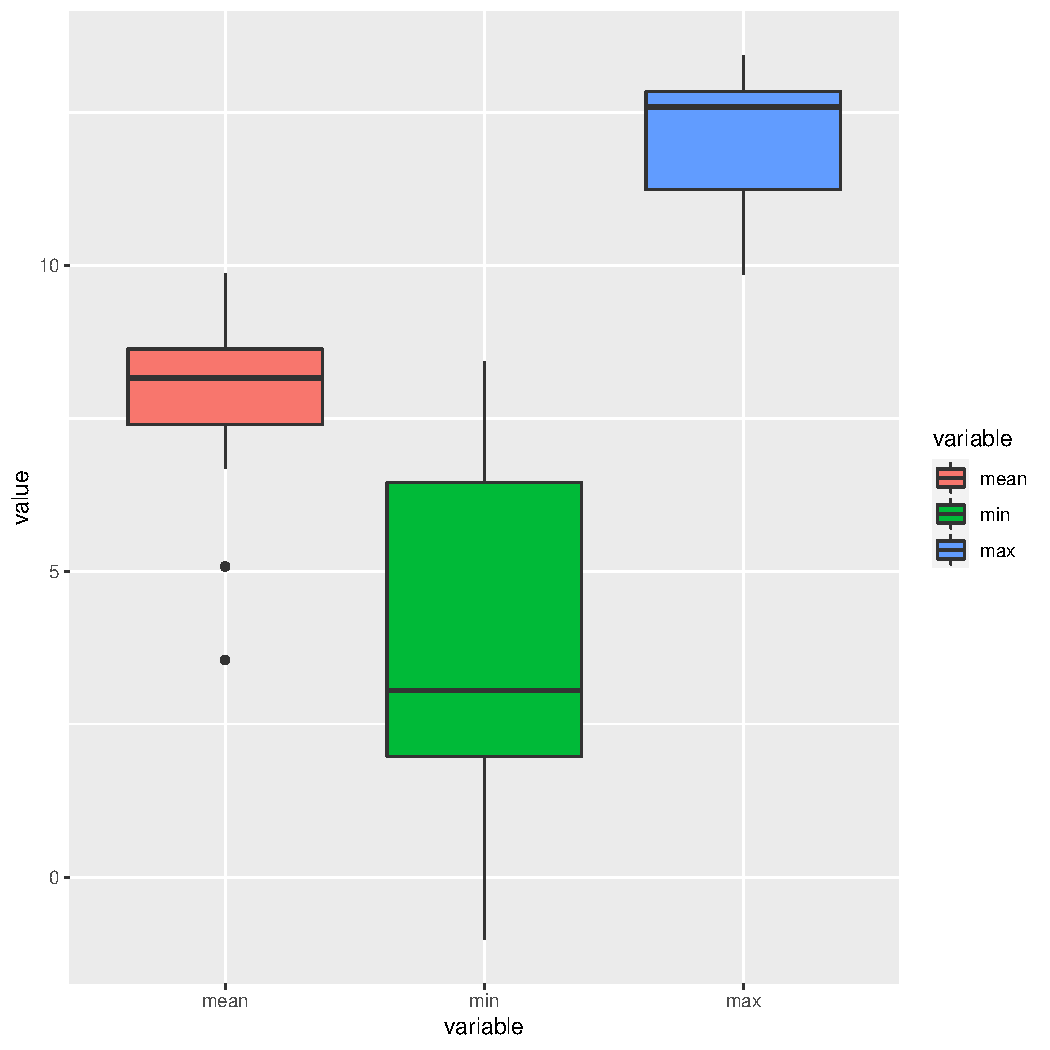
\includegraphics[width=.5\textwidth]{./figures/example_analysis}
    \caption{Boxplot of the mean, minimum and maximum hourly, quality checked air temperature in Freiburg on Christmas eve. The data was taken from 52 different locations in 2019, 2020 and 2021. Original measurements were taken with an onset HOBO temperature data logger.}
    \label{fig:first_figure}
\end{figure}

% REPLACE WITH YOUR TEXT HERE
This last section should focus on the question how this years' measurements compare 
to the last few years. For this, you are asked to produce a number of graphs. 
The best practice is to generate PDF graphics and include them directly here.
The necessary commands are already loaded in this template.

You can even automate your workflow further and run your scripts producing the 
PDFs in this repository, saving them to the \texttt{'./figures/'} subfolder. 
This will refresh the figures in the report whenever, your scripts overwrite them (Fig \ref{fig:first_figure}).

The figure above can be included like:

\begin{verbatim}
\begin{figure}[ht]
    \centering
    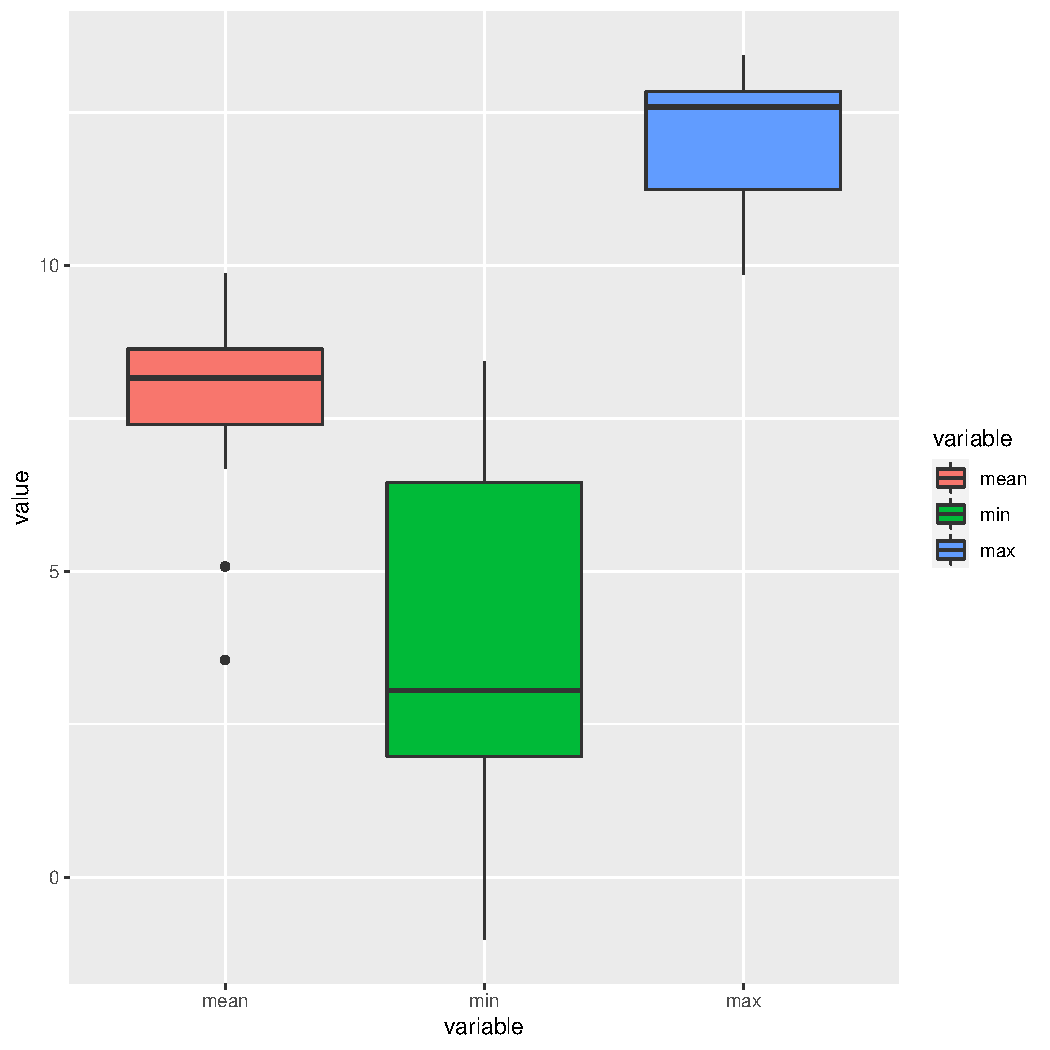
\includegraphics[width=.5\textwidth]{./figures/example_analysis}
    \caption{Boxplot of the mean, minimum and maximum hourly, quality 
    checked air temperature in Freiburg on Christmas eve. The data was 
    taken from 52 different locations in 2019, 2020 and 2021. Original 
    measurements were taken with an onset HOBO temperature data logger.}
    \label{fig:first_figure}
\end{figure}
\end{verbatim}




%\wordcount{main}

\bibliography{bibliography}
\end{document}